% !TEX program = xelatex
\documentclass[11pt,italian,a4paper]{article}

\usepackage{fancyhdr}
\usepackage[a4paper, total={6.5in, 9.5in}]{geometry}
\usepackage{fontspec}
\usepackage[utf8]{inputenc}
\usepackage[T1]{fontenc}
\usepackage{foreign}
\usepackage[american]{babel}
\usepackage[export]{adjustbox}
\usepackage{ragged2e}
\usepackage{xurl}
\usepackage{hyperref}
\usepackage{titlesec}
\usepackage{amsmath}
\usepackage{graphicx,floatpag,caption}
\usepackage{rotating}
\usepackage{blindtext}
\usepackage{pst-plot}
\usepackage{pgfplots}
\usepackage[table]{xcolor}
\usepackage{wrapfig}
\usepackage{multirow}
\usepackage{stackengine}
\usepackage{pdflscape}
\usepackage{draftwatermark}
\usepackage{tcolorbox}
\usepackage{float}
\usepackage{fontawesome5}
\usepackage{listings}

\SetWatermarkText{DRAFT}
\SetWatermarkScale{1}
\SetWatermarkLightness{0.9}

\hypersetup{
    colorlinks,
    linkcolor={red!50!black},
    citecolor={blue!50!black},
    urlcolor={blue!80!black}
}

\definecolor{violettissimo}{RGB}{159, 116, 183}
\definecolor{violettinissimo}{RGB}{207, 185, 219}
\definecolor{verde}{RGB}{102, 153, 0}

\renewcommand{\familydefault}{\sfdefault}

\pagenumbering{arabic}
\title{Computer Science & Engineering Project}
\author{Alessandro Modica (10822654 / 212683)}
\pagestyle{fancy}
\date{6 aprile 2025}

\fancyfoot[C]{\thepage}

\newcommand{\todo}[1]{\noindent {\Huge \color{orange} TODO -- #1}}
\newcommand{\inlineicon}[1]{\raisebox{-.25\height}{\includegraphics[height=\baselineskip,keepaspectratio]{figures/icons/#1}}}

\begin{document}
\begin{titlepage}
    \begin{center}

        \Huge{Computer Engineering Project Report}\\
        \vspace*{0.5cm}
        \Huge\textbf{Ludika}\\
        \LARGE\textbf{A Platform for Game-Based Learning Tools Assessment}\\

        \vspace*{2cm}

        % \rule[0.5ex]{\textwidth}{0.5pt} \\
        \adjincludegraphics[width=0.8\textwidth]{figures/ludika-api-swagger.png} \\
        \rule[0.5ex]{\textwidth}{0.5pt}


        \vspace*{2cm}

        \begin{minipage}{0.6\textwidth}
            \begin{flushleft}
                \Large\noindent{Made by \textbf{Alessandro Modica} \\ Supervising Professor \textbf{Fabrizio Amarilli}}
            \end{flushleft}
        \end{minipage}
        \begin{minipage}{0.35\textwidth}
            \begin{flushright}
                \Large\noindent\textbf{July 27, 2025}
            \end{flushright}
        \end{minipage}

    \end{center}

    \vfill

    \begin{minipage}{0.7\textwidth}
        \begin{minipage}{0.5\textwidth}
            \centering
            {\huge Report made with}\vspace{0.3em} {\Huge \LaTeX}
        \end{minipage}
    \end{minipage}
    \begin{minipage}{0.3\textwidth}
        \flushright
        
\includegraphics[width=\textwidth]{figures/Logo_Politecnico_Milano.png}
    \end{minipage}
\end{titlepage}

\tableofcontents

\setlength{\parskip}{0.5em}

\section{Introduction}

Game-Based Learning (GBL) is a pedagogical approach that uses games to enhance the learning experience. It has been shown to improve student engagement, motivation, and retention of knowledge. A significant market at \$US 14.0 billion in 2023\footnote{\href{https://market.us/report/game-based-learning-market/}{Global Game-Based Learning Market Size, Share, Trends Analysis Report By Component (Solution, and Services), By Game Type (AR VR Games, AI-based Games, and Training, Knowledge \& Skill-based games, language learning games, and others), By Deployment Type (On-Premises, and Cloud), By End-User, By Region and Companies - Industry Segment Outlook, Market Assessment, Competition Scenario, Trends and Forecast 2023-2032}}, it is projected to grow significantly in the coming years.

The growing prevalence of online learning and game-based educational tools has led many teachers and institutions to seek ways to determine the effectiveness of these tools in improving student learning outcomes. This project aims to develop a platform to enable a more systematic and data-driven approach to indexing, evaluating and discovering the best game-based learning tools.


\begin{figure}[h]
    \centering
    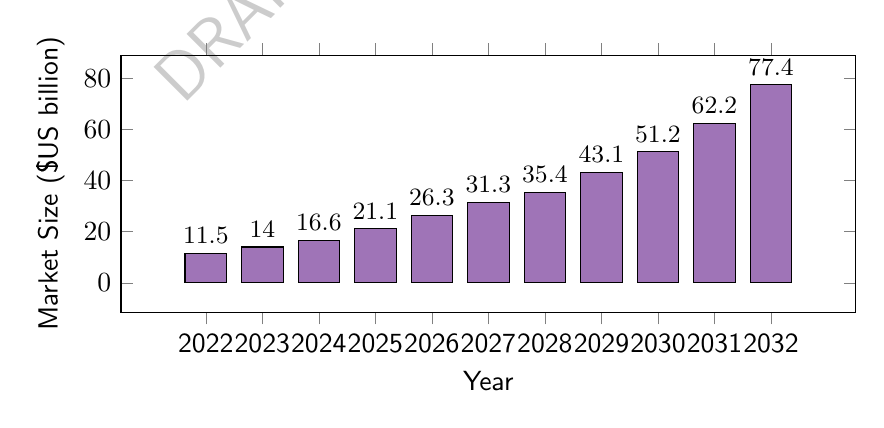
\begin{tikzpicture}
        \begin{axis}[
                width=0.9\textwidth,
                height=0.4\textwidth,
                ybar,
                bar width=15pt,
                enlargelimits=0.15,
                ylabel={Market Size (\$US billion)},
                xlabel={Year},
                symbolic x coords={2022,2023,2024,2025,2026,2027,2028,2029,2030,2031,2032},
                xtick=data,
                ymin=0,
                nodes near coords,
                nodes near coords align={vertical},
                every node near coord/.append style={font=\small},
            ]
            \addplot[fill=violettissimo] coordinates {(2022,11.5) (2023,14.0) (2024,16.6) (2025,21.1) (2026,26.3) (2027,31.3) (2028,35.4) (2029,43.1) (2030,51.2) (2031,62.2) (2032,77.4)};
        \end{axis}
    \end{tikzpicture}
    \caption{Growth of the Game-Based Learning Market, including the projected growth till 2032.}
\end{figure}

Through a sleek user-friendly web interface, teachers and students alike can easily browse, cross-compare, suggest and review various educational games. The platform will also provide a set of metrics and analytics to help teachers gauge the effectiveness of these tools in their classrooms. Native integration with the API of OpenAI-compatible Large Language Models (LLMs) allows for interactive, AI-facilitated categorization and addition of new games, as well as the generation of summaries, comparisons, and personalized recommendations based on user requirements.

Given diverging priorities and needs, teachers greatly benefit from the ability to use Multi-Criteria Decision Making (MCDM) and Weighted Ranking methods to evaluate and compare educational games. The platform will allow teachers to create custom evaluation criteria, assign weights to each criterion, and then rank the games based on their performance against these criteria.

In order to achieve these goals, the project was developed using a three-tier architecture with the API and backend logic contained within a monolithic service, in order to attain the best efficiency and reduce the footprint of service interoperation logic. The platform is built using state-of-the-art web technologies, including Nuxt for the frontend, FastAPI for the backend, and PostgreSQL for the database. Langchain provides the backbone for agentic features, while evaluations are algorithmically generated based on the games' metadata and user reviews.

The use of Docker allows for easy deployment and management of the various components of the system, and native integration with Cloudflare enables the use of a CDN for fast and reliable content delivery.

\todo{add high-level information on the development timeline and background.}

\section{Related Work---a comparative overview}
\todo{add a comparative analysis of the most similar existing platforms, and/or relevant studies that have been conducted in the past.}

\section{Innovation of the proposed solution}

The core value-add of the proposed solution is the tight integration of all the core components (game discovery, agentic web scraping, bespoke ranking algorithms and the fine-tuned game indexing and fuzzy search systems) into a single platform. In particular, the ability for teachers to define their own criteria makes using this platform more helpful, relevant and personal than any experience possible using a generic off-the-shelf CMS solution like Wordpress.

With the default criteria provided, teachers are able to compare their own preferences with those of their colleagues by seeing how the same game ranks under different sets of weights, allowing them to make more informed decisions about which games to use in their classrooms.

This platform is intended to be a living, breathing tool that evolves with the needs of its users. It has a community-driven approach to development, enabling administrators to take in suggestions and feedback from users and extend categorization and evaluation options as needed.

\section{Project Development}

In this section, I will provide an in-depth overview of the development process, including the rationale behind design choices, specifics about the implementation of the platform, as well as the challenges faced and lessons learned along the way.

\subsection{Functionality}

The platform implements a set of core functionalities that allow \textbf{\textit{Users}} to:

\begin{itemize}
    \item \textbf{browse and search} for educational games, either by using a search bar or by filtering through a set of predefined categories;
    \item \textbf{compare} educational games based on a set of criteria, including user reviews, ratings, and other relevant metrics;
    \item \textbf{evaluate} educational games using a set of custom criteria defined by the user, allowing for a more personalized and relevant experience;
    \item \textbf{submit} new educational games to the platform as suggestions, allowing moderators to review and approve them;
    \item \textbf{review} educational games, providing feedback and ratings to help other users make informed decisions;
    \item \textbf{generate} personalized recommendations based on user preferences and requirements, using natural language queries to be processed by OpenAI-compatible Large Language Models (LLMs) and a dedicated agentic recommendation engine.
\end{itemize}

\noindent Additonally, \textbf{\textit{Content Moderators}} and \textbf{\textit{Platform Administrators}} are able to:
\begin{itemize}
    \item \textbf{add} new educational games to the platform, either by using a web form or by using the agentic web scraping feature;
    \item \textbf{approve} or reject user-submitted educational games, ensuring that only high-quality and relevant content is available on the platform;
    \item \textbf{manage} user contents and accounts, including the ability to ban or suspend users who violate the platform's terms of service;
    \item \textbf{monitor} user activity and engagement, providing insights into how users are interacting with the platform and which games are most popular.
\end{itemize}

\todo{review featureset to ensure it is complete, while evaluating the feasibility of implementing all features.}

\subsection{Technology Stack}
The platform is built upon a robust technology stack that includes:

\begin{itemize}
    \item \textbf{Frontend:} \inlineicon{nuxt.png} \href{https://nuxt.com/}{Nuxt}, a powerful framework for building responsive server-rendered applications with Vue, providing a seamless user experience and fast performance. Presentation layer processing is thus partly offloaded to the server, allowing for faster page loads and improved SEO. Nuxt is built on top of Vue, a popular JavaScript framework for building user interfaces, and provides a powerful set of features for building applications for the modern web.
    \item \textbf{Backend:} \inlineicon{fastapi.png} \href{https://fastapi.tiangolo.com/}{FastAPI}, a modern web framework for building APIs with Python based on standard Python type hints, first-class citizen support for Pydantic models and an asynchronous runtime conforming to the ASGI standard, ensuring high performance and easy development.
    \item \textbf{Database:} \inlineicon{postgres.png} \href{https://www.postgresql.org/}{PostgreSQL}, a powerful open-source relational database system that provides reliability and data integrity. Its advanced features, such as support for JSON object storage, full-text search and concurrency synchronization semantics via \textit{advisory locks}, make it an ideal choice for this project.
    \item \textbf{Containerization:} \inlineicon{docker.png} \href{https://www.docker.com/}{Docker}, allowing for easy deployment and management of the various components of the system. Docker implements the OCI runtime specification, which allows for the use of OCI-compliant container images and runtimes in any environment that supports the OCI standard, such as Kubernetes, OpenShift, Amazon ECS, and Azure Container Instances.
    \item \textbf{ORM:} \inlineicon{sqlmodel.png} \href{https://sqlmodel.tiangolo.com/}{SQLModel}, a Python library that provides a simple and efficient way to interact with databases using Python objects. It is built on top of SQLAlchemy and Pydantic, providing a powerful and flexible ORM solution for FastAPI applications reducing code repetition and improving maintainability.
    \item \textbf{Web Scraping:} \inlineicon{scrapy.png} \href{https://scrapy.org/}{Scrapy}, a Python library for web scraping that allows for easy extraction of data from HTML and XML documents. It provides a powerful and flexible framework for building web crawlers and spiders, making it easy to discover and index new educational games reducing the need for manual input.
    \item \textbf{CDN:} \inlineicon{cloudflare.png} \href{https://www.cloudflare.com/}{Cloudflare}, providing fast and reliable content delivery through its global network.
    \item \textbf{LLM Integration:} \inlineicon{langchain.png} \href{https://www.langchain.com/}{Langchain}, enabling the use of OpenAI-compatible Large Language Models for interactive categorization and personalized recommendations.
\end{itemize}

\subsection{Architecture}

\todo{add a diagram of the architecture of the platform, including the various components and how they interact with each other. Will be included once the project can be deployed and tested.}

\subsubsection{Data Model}

\begin{figure}[H]
    \centering
    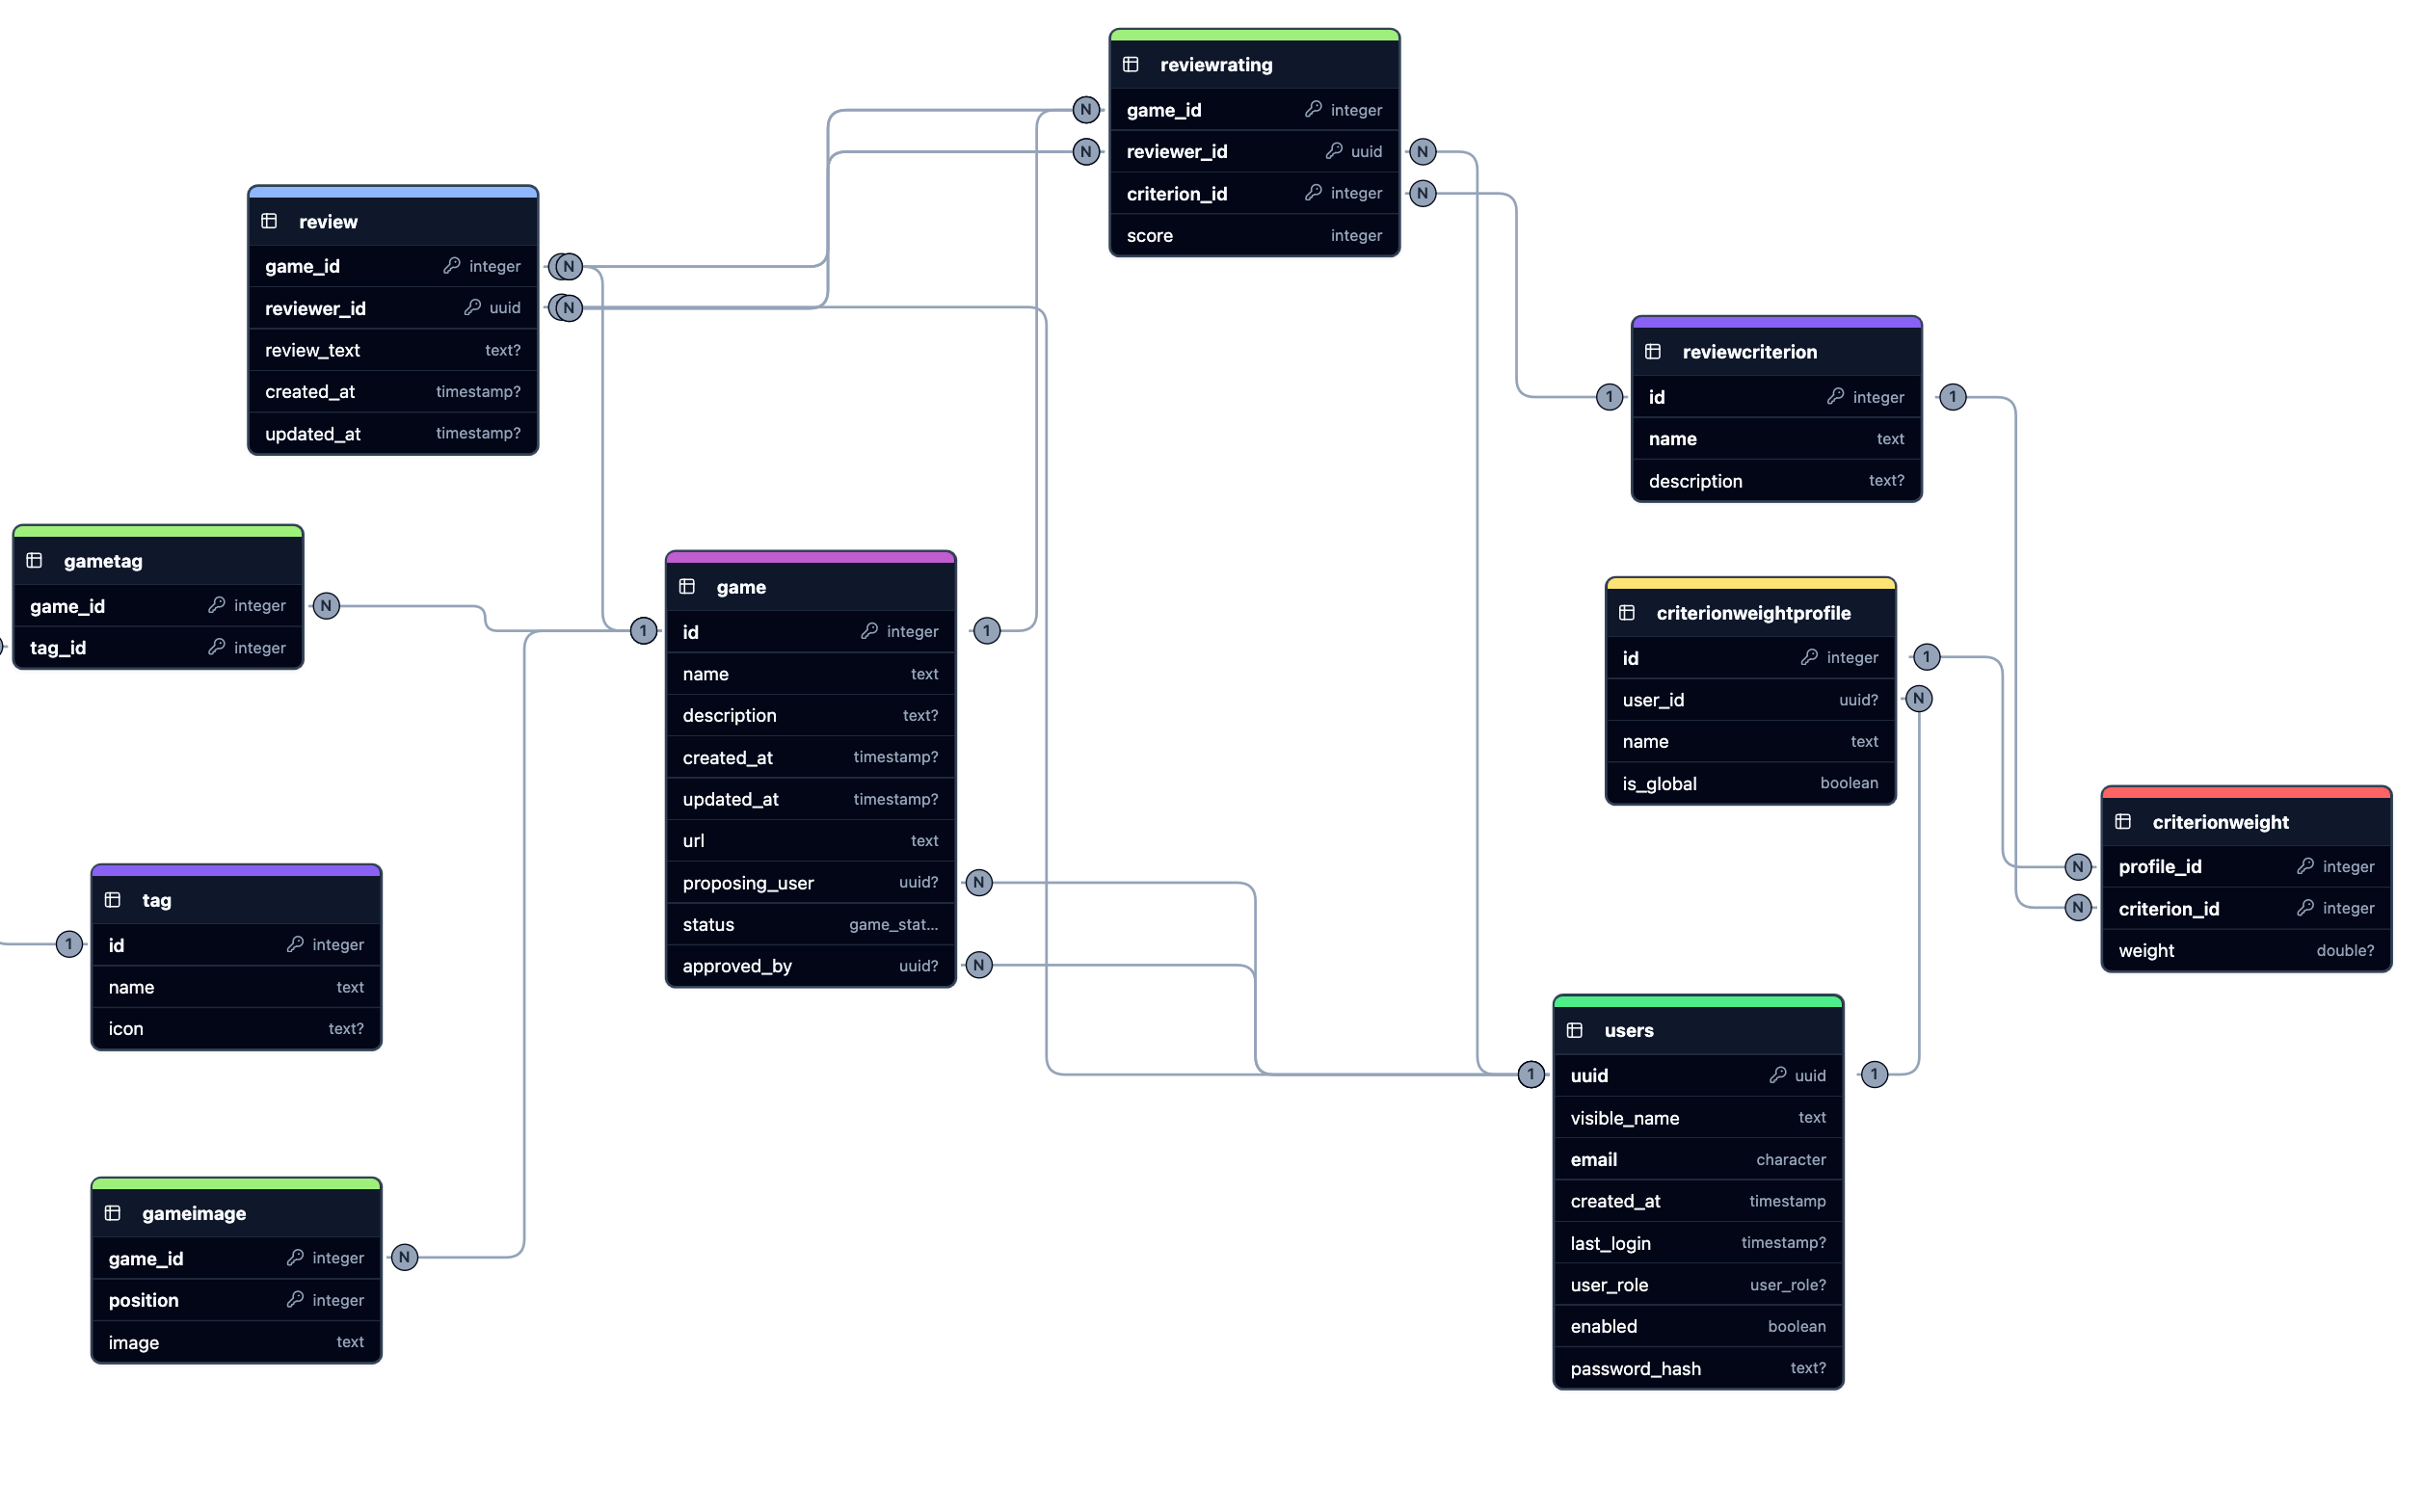
\includegraphics[width=\textwidth]{figures/data_model.png}
    \caption{Data Model}
\end{figure}

The data model is designed with efficiency and simplicity in mind, using SQL--native constraints and indexes to ensure maximum performance. The following entities and relations are defined:

\begin{itemize}
    \item \textbf{Users}: Registered accounts, each with a unique UUID, visible name, email, creation and last login timestamps, a user role (\texttt{user}, \texttt{content\_moderator}, or \texttt{platform\_administrator}), enabled status, and password hash. Disabled users are prevented from logging in.
    \item \textbf{Game}: Educational games proposed by users, with fields for name, description, creation and update timestamps, URL, proposing user, status (\texttt{draft}, \texttt{submitted}, \texttt{approved}, or \texttt{rejected}), and the approving user.
    \item \textbf{GameImage}: Images associated with each game, identified by game ID and position, storing the image path or reference.
    \item \textbf{Tag}: Tags that can be assigned to games, each with an ID, name, and optional icon. Tags are used to categorize games and allow for easy filtering and searching.
    \item \textbf{GameTag}: Association table linking games and tags (many-to-many relationship).
    \item \textbf{ReviewCriterion}: Criteria used for reviewing games (e.g., ``Ease of use'', ``Fun factor''), each with a unique name and description.
    \item \textbf{Review}: Reviews of games by users, including review text, creation and update timestamps, and identified by game and reviewer.
    \item \textbf{ReviewRating}: Ratings for each criterion in a review, storing the score (1--5) for each criterion, game, and reviewer.
    \item \textbf{CriterionWeightProfile}: Weight profiles defined by users (or admins if global), with a name and a flag indicating if the profile is global.
    \item \textbf{CriterionWeight}: Weights for each criterion in a weight profile, associating a profile with a criterion and a non-negative weight.
\end{itemize}

\noindent The project also makes use of the following custom PostgreSQL enum types:
\begin{itemize}
    \item \texttt{user\_role}: \{\texttt{user}, \texttt{content\_moderator}, \texttt{platform\_administrator}\}
    \item \texttt{game\_status}: \{\texttt{draft}, \texttt{submitted}, \texttt{approved}, \texttt{rejected}\}
\end{itemize}


\subsubsection{API Model}

The API, built using FastAPI, uses a RESTful architecture with JSON responses, Bearer authentication and OpenAPI documentation. The following endpoints are available:

%%%
%%% This is an automatically generated file. Do not edit!
%%% Generated by apissima.py
%%% To (re-)build:
%%%
%%%   cd ludika-backend/
%%%   source .venv/bin/activate
%%%   # ensure valid configuration and dependencies exist for ludika-backend
%%%   python ../ludika-docs/tools/apissima.py
%%%
%%% followed by rebuilding the documentation with XeTeX. 
%%%

\textbullet\ \texttt{/}:\begin{tcolorbox}[colback=violettissimo!10!white, colframe=violettissimo, title=\textbf{GET /} --- Status, fonttitle=\bfseries, sharp corners=south, boxrule=0.8pt, left=2mm, right=2mm, top=1mm, bottom=1mm]\textbf{Description:} Root endpoint that returns status information.\\
\textbf{Response:} \texttt{application/json (json)}\end{tcolorbox}


\textbullet\ \texttt{/status}:\begin{tcolorbox}[colback=violettissimo!10!white, colframe=violettissimo, title=\textbf{GET /status} --- Status, fonttitle=\bfseries, sharp corners=south, boxrule=0.8pt, left=2mm, right=2mm, top=1mm, bottom=1mm]\textbf{Description:} Root endpoint that returns status information.\\
\textbf{Response:} \texttt{application/json (json)}\end{tcolorbox}


\textbullet\ \texttt{/games/}:\begin{tcolorbox}[colback=violettissimo!10!white, colframe=violettissimo, title=\textbf{GET /games/} --- Get Games, fonttitle=\bfseries, sharp corners=south, boxrule=0.8pt, left=2mm, right=2mm, top=1mm, bottom=1mm]\textbf{Description:} Retrieve a list of all approved games with pagination, tag filtering and search.\\
\textbf{Response:} \texttt{application/json (json)}\end{tcolorbox}
\begin{tcolorbox}[colback=verde!10!white, colframe=verde, title=\textbf{\faLock{} POST /games/} --- Create Game, fonttitle=\bfseries, sharp corners=south, boxrule=0.8pt, left=2mm, right=2mm, top=1mm, bottom=1mm]\textbf{Description:} Create a new game.\\
\textbf{Request Body:} \texttt{application/json}\\
\textbf{Response:} \texttt{application/json (json)}\end{tcolorbox}


\textbullet\ \texttt{/games/my-games}:\begin{tcolorbox}[colback=violettissimo!10!white, colframe=violettissimo, title=\textbf{\faLock{} GET /games/my-games} --- Get My Games, fonttitle=\bfseries, sharp corners=south, boxrule=0.8pt, left=2mm, right=2mm, top=1mm, bottom=1mm]\textbf{Description:} Get games created by the current user.\\
\textbf{Response:} \texttt{application/json (json)}\end{tcolorbox}


\textbullet\ \texttt{/games/waiting-for-approval}:\begin{tcolorbox}[colback=violettissimo!10!white, colframe=violettissimo, title=\textbf{\faLock{} GET /games/waiting-for-approval} --- Get Games Waiting For Approval, fonttitle=\bfseries, sharp corners=south, boxrule=0.8pt, left=2mm, right=2mm, top=1mm, bottom=1mm]\textbf{Description:} Get games waiting for approval (privileged users only).\\
\textbf{Response:} \texttt{application/json (json)}\end{tcolorbox}


\textbullet\ \texttt{/games/\string{game\_id\string}}:\begin{tcolorbox}[colback=violettissimo!10!white, colframe=violettissimo, title=\textbf{\faLock{} GET /games/\string{game\_id\string}} --- Get Game, fonttitle=\bfseries, sharp corners=south, boxrule=0.8pt, left=2mm, right=2mm, top=1mm, bottom=1mm]\textbf{Description:} Retrieve a game by its ID.\\
\textbf{Response:} \texttt{application/json (json)}\end{tcolorbox}
\begin{tcolorbox}[colback=red!10!white, colframe=red, title=\textbf{\faLock{} DELETE /games/\string{game\_id\string}} --- Delete Game, fonttitle=\bfseries, sharp corners=south, boxrule=0.8pt, left=2mm, right=2mm, top=1mm, bottom=1mm]\textbf{Description:} Delete a game (only by creator or privileged users).\\
\textbf{Response:} \texttt{application/json (json)}\end{tcolorbox}
\begin{tcolorbox}[colback=purple!10!white, colframe=purple, title=\textbf{\faLock{} PATCH /games/\string{game\_id\string}} --- Update Game, fonttitle=\bfseries, sharp corners=south, boxrule=0.8pt, left=2mm, right=2mm, top=1mm, bottom=1mm]\textbf{Description:} Update a game (only by creator or privileged users).\\
\textbf{Request Body:} \texttt{application/json}\\
\textbf{Response:} \texttt{application/json (json)}\end{tcolorbox}


\textbullet\ \texttt{/games/\string{game\_id\string}/with-reviews}:\begin{tcolorbox}[colback=violettissimo!10!white, colframe=violettissimo, title=\textbf{\faLock{} GET /games/\string{game\_id\string}/with-reviews} --- Get Game With Reviews, fonttitle=\bfseries, sharp corners=south, boxrule=0.8pt, left=2mm, right=2mm, top=1mm, bottom=1mm]\textbf{Description:} Retrieve a game by its ID with reviews included.\\
\textbf{Response:} \texttt{application/json (json)}\end{tcolorbox}


\textbullet\ \texttt{/games/\string{game\_id\string}/images/\string{image\_no\string}}:\begin{tcolorbox}[colback=violettissimo!10!white, colframe=violettissimo, title=\textbf{\faLock{} GET /games/\string{game\_id\string}/images/\string{image\_no\string}} --- Get Game Image, fonttitle=\bfseries, sharp corners=south, boxrule=0.8pt, left=2mm, right=2mm, top=1mm, bottom=1mm]\textbf{Description:} Get a specific image for a game.\\
\textbf{Response:} \texttt{application/json (json)}\end{tcolorbox}
\begin{tcolorbox}[colback=orange!10!white, colframe=orange, title=\textbf{\faLock{} PUT /games/\string{game\_id\string}/images/\string{image\_no\string}} --- Replace Game Image, fonttitle=\bfseries, sharp corners=south, boxrule=0.8pt, left=2mm, right=2mm, top=1mm, bottom=1mm]\textbf{Description:} Replace an existing image for a game.\\
\textbf{Request Body:} \texttt{multipart/form-data}\\
\textbf{Response:} \texttt{application/json (json)}\end{tcolorbox}
\begin{tcolorbox}[colback=red!10!white, colframe=red, title=\textbf{\faLock{} DELETE /games/\string{game\_id\string}/images/\string{image\_no\string}} --- Delete Game Image, fonttitle=\bfseries, sharp corners=south, boxrule=0.8pt, left=2mm, right=2mm, top=1mm, bottom=1mm]\textbf{Description:} Delete a specific image from a game.\\
\textbf{Response:} \texttt{application/json (json)}\end{tcolorbox}


\textbullet\ \texttt{/games/\string{game\_id\string}/images}:\begin{tcolorbox}[colback=verde!10!white, colframe=verde, title=\textbf{\faLock{} POST /games/\string{game\_id\string}/images} --- Post Game Image, fonttitle=\bfseries, sharp corners=south, boxrule=0.8pt, left=2mm, right=2mm, top=1mm, bottom=1mm]\textbf{Description:} Upload a new image for a game.\\
\textbf{Request Body:} \texttt{multipart/form-data}\\
\textbf{Response:} \texttt{application/json (json)}\end{tcolorbox}


\textbullet\ \texttt{/games/ranked/\string{profile\_id\string}}:\begin{tcolorbox}[colback=violettissimo!10!white, colframe=violettissimo, title=\textbf{\faLock{} GET /games/ranked/\string{profile\_id\string}} --- Get Ranked Games, fonttitle=\bfseries, sharp corners=south, boxrule=0.8pt, left=2mm, right=2mm, top=1mm, bottom=1mm]\textbf{Description:} Get ranked games for a given profile.\\
\textbf{Response:} \texttt{application/json (json)}\end{tcolorbox}


\textbullet\ \texttt{/tags/}:\begin{tcolorbox}[colback=violettissimo!10!white, colframe=violettissimo, title=\textbf{GET /tags/} --- Get Tags, fonttitle=\bfseries, sharp corners=south, boxrule=0.8pt, left=2mm, right=2mm, top=1mm, bottom=1mm]\textbf{Description:} Get all tags.\\
\textbf{Response:} \texttt{application/json (json)}\end{tcolorbox}
\begin{tcolorbox}[colback=verde!10!white, colframe=verde, title=\textbf{\faLock{} POST /tags/} --- Add Tag, fonttitle=\bfseries, sharp corners=south, boxrule=0.8pt, left=2mm, right=2mm, top=1mm, bottom=1mm]\textbf{Description:} Create a new tag (admin only).\\
\textbf{Request Body:} \texttt{application/json}\\
\textbf{Response:} \texttt{application/json (json)}\end{tcolorbox}


\textbullet\ \texttt{/tags/\string{tag\_id\string}}:\begin{tcolorbox}[colback=red!10!white, colframe=red, title=\textbf{\faLock{} DELETE /tags/\string{tag\_id\string}} --- Delete Tag, fonttitle=\bfseries, sharp corners=south, boxrule=0.8pt, left=2mm, right=2mm, top=1mm, bottom=1mm]\textbf{Description:} Delete a tag (admin only).\\
\textbf{Response:} \texttt{application/json (json)}\end{tcolorbox}
\begin{tcolorbox}[colback=purple!10!white, colframe=purple, title=\textbf{\faLock{} PATCH /tags/\string{tag\_id\string}} --- Update Tag, fonttitle=\bfseries, sharp corners=south, boxrule=0.8pt, left=2mm, right=2mm, top=1mm, bottom=1mm]\textbf{Description:} Update a tag (admin only).\\
\textbf{Request Body:} \texttt{application/json}\\
\textbf{Response:} \texttt{application/json (json)}\end{tcolorbox}


\textbullet\ \texttt{/users/}:\begin{tcolorbox}[colback=violettissimo!10!white, colframe=violettissimo, title=\textbf{\faLock{} GET /users/} --- List Users, fonttitle=\bfseries, sharp corners=south, boxrule=0.8pt, left=2mm, right=2mm, top=1mm, bottom=1mm]\textbf{Description:} Get all users (privileged users only).\\
\textbf{Response:} \texttt{application/json (json)}\end{tcolorbox}


\textbullet\ \texttt{/users/me}:\begin{tcolorbox}[colback=violettissimo!10!white, colframe=violettissimo, title=\textbf{\faLock{} GET /users/me} --- Get Me, fonttitle=\bfseries, sharp corners=south, boxrule=0.8pt, left=2mm, right=2mm, top=1mm, bottom=1mm]\textbf{Description:} Get the current user.\\
\textbf{Response:} \texttt{application/json (json)}\end{tcolorbox}


\textbullet\ \texttt{/users/me/visible-name}:\begin{tcolorbox}[colback=purple!10!white, colframe=purple, title=\textbf{\faLock{} PATCH /users/me/visible-name} --- Update Visible Name, fonttitle=\bfseries, sharp corners=south, boxrule=0.8pt, left=2mm, right=2mm, top=1mm, bottom=1mm]\textbf{Description:} Update the current user's visible name.\\
\textbf{Request Body:} \texttt{application/json}\\
\textbf{Response:} \texttt{application/json (json)}\end{tcolorbox}


\textbullet\ \texttt{/users/me/password}:\begin{tcolorbox}[colback=purple!10!white, colframe=purple, title=\textbf{\faLock{} PATCH /users/me/password} --- Update Password, fonttitle=\bfseries, sharp corners=south, boxrule=0.8pt, left=2mm, right=2mm, top=1mm, bottom=1mm]\textbf{Description:} Update the current user's password.\\
\textbf{Request Body:} \texttt{application/json}\\
\textbf{Response:} \texttt{application/json (json)}\end{tcolorbox}


\textbullet\ \texttt{/users/\string{user\_id\string}}:\begin{tcolorbox}[colback=violettissimo!10!white, colframe=violettissimo, title=\textbf{\faLock{} GET /users/\string{user\_id\string}} --- Get User, fonttitle=\bfseries, sharp corners=south, boxrule=0.8pt, left=2mm, right=2mm, top=1mm, bottom=1mm]\textbf{Description:} Get a specific user by ID (privileged users only).\\
\textbf{Response:} \texttt{application/json (json)}\end{tcolorbox}
\begin{tcolorbox}[colback=purple!10!white, colframe=purple, title=\textbf{\faLock{} PATCH /users/\string{user\_id\string}} --- Admin Update User, fonttitle=\bfseries, sharp corners=south, boxrule=0.8pt, left=2mm, right=2mm, top=1mm, bottom=1mm]\textbf{Description:} Update a user (privileged users only).\\
\textbf{Request Body:} \texttt{application/json}\\
\textbf{Response:} \texttt{application/json (json)}\end{tcolorbox}
\begin{tcolorbox}[colback=red!10!white, colframe=red, title=\textbf{\faLock{} DELETE /users/\string{user\_id\string}} --- Delete User, fonttitle=\bfseries, sharp corners=south, boxrule=0.8pt, left=2mm, right=2mm, top=1mm, bottom=1mm]\textbf{Description:} Delete a user (admin only).\\
\textbf{Response:} \texttt{application/json (json)}\end{tcolorbox}


\textbullet\ \texttt{/users/\string{user\_id\string}/games}:\begin{tcolorbox}[colback=red!10!white, colframe=red, title=\textbf{\faLock{} DELETE /users/\string{user\_id\string}/games} --- Delete User Games, fonttitle=\bfseries, sharp corners=south, boxrule=0.8pt, left=2mm, right=2mm, top=1mm, bottom=1mm]\textbf{Description:} Delete all games created by a user (moderators and admins only).\\
\textbf{Response:} \texttt{application/json (json)}\end{tcolorbox}


\textbullet\ \texttt{/reviews/criteria}:\begin{tcolorbox}[colback=violettissimo!10!white, colframe=violettissimo, title=\textbf{GET /reviews/criteria} --- List Criteria, fonttitle=\bfseries, sharp corners=south, boxrule=0.8pt, left=2mm, right=2mm, top=1mm, bottom=1mm]\textbf{Description:} Get all review criteria.\\
\textbf{Response:} \texttt{application/json (json)}\end{tcolorbox}
\begin{tcolorbox}[colback=verde!10!white, colframe=verde, title=\textbf{\faLock{} POST /reviews/criteria} --- Create Criterion, fonttitle=\bfseries, sharp corners=south, boxrule=0.8pt, left=2mm, right=2mm, top=1mm, bottom=1mm]\textbf{Description:} Create a new review criterion (admin only).\\
\textbf{Request Body:} \texttt{application/json}\\
\textbf{Response:} \texttt{application/json (json)}\end{tcolorbox}


\textbullet\ \texttt{/reviews/criteria/\string{criterion\_id\string}}:\begin{tcolorbox}[colback=purple!10!white, colframe=purple, title=\textbf{\faLock{} PATCH /reviews/criteria/\string{criterion\_id\string}} --- Update Criterion, fonttitle=\bfseries, sharp corners=south, boxrule=0.8pt, left=2mm, right=2mm, top=1mm, bottom=1mm]\textbf{Description:} Update a review criterion (admin only).\\
\textbf{Request Body:} \texttt{application/json}\\
\textbf{Response:} \texttt{application/json (json)}\end{tcolorbox}
\begin{tcolorbox}[colback=red!10!white, colframe=red, title=\textbf{\faLock{} DELETE /reviews/criteria/\string{criterion\_id\string}} --- Delete Criterion, fonttitle=\bfseries, sharp corners=south, boxrule=0.8pt, left=2mm, right=2mm, top=1mm, bottom=1mm]\textbf{Description:} Delete a review criterion (admin only).\\
\textbf{Response:} \texttt{application/json (json)}\end{tcolorbox}


\textbullet\ \texttt{/reviews/profiles}:\begin{tcolorbox}[colback=violettissimo!10!white, colframe=violettissimo, title=\textbf{\faLock{} GET /reviews/profiles} --- List Profiles, fonttitle=\bfseries, sharp corners=south, boxrule=0.8pt, left=2mm, right=2mm, top=1mm, bottom=1mm]\textbf{Description:} Get available criterion weight profiles.\\
\textbf{Response:} \texttt{application/json (json)}\end{tcolorbox}
\begin{tcolorbox}[colback=verde!10!white, colframe=verde, title=\textbf{\faLock{} POST /reviews/profiles} --- Create Profile, fonttitle=\bfseries, sharp corners=south, boxrule=0.8pt, left=2mm, right=2mm, top=1mm, bottom=1mm]\textbf{Description:} Create a new criterion weight profile.\\
\textbf{Request Body:} \texttt{application/json}\\
\textbf{Response:} \texttt{application/json (json)}\end{tcolorbox}


\textbullet\ \texttt{/reviews/profiles/\string{profile\_id\string}}:\begin{tcolorbox}[colback=violettissimo!10!white, colframe=violettissimo, title=\textbf{\faLock{} GET /reviews/profiles/\string{profile\_id\string}} --- Get Profile, fonttitle=\bfseries, sharp corners=south, boxrule=0.8pt, left=2mm, right=2mm, top=1mm, bottom=1mm]\textbf{Description:} Get a criterion weight profile.\\
\textbf{Response:} \texttt{application/json (json)}\end{tcolorbox}
\begin{tcolorbox}[colback=purple!10!white, colframe=purple, title=\textbf{\faLock{} PATCH /reviews/profiles/\string{profile\_id\string}} --- Update Profile, fonttitle=\bfseries, sharp corners=south, boxrule=0.8pt, left=2mm, right=2mm, top=1mm, bottom=1mm]\textbf{Description:} Update a criterion weight profile.\\
\textbf{Request Body:} \texttt{application/json}\\
\textbf{Response:} \texttt{application/json (json)}\end{tcolorbox}
\begin{tcolorbox}[colback=red!10!white, colframe=red, title=\textbf{\faLock{} DELETE /reviews/profiles/\string{profile\_id\string}} --- Delete Profile, fonttitle=\bfseries, sharp corners=south, boxrule=0.8pt, left=2mm, right=2mm, top=1mm, bottom=1mm]\textbf{Description:} Delete a criterion weight profile.\\
\textbf{Response:} \texttt{application/json (json)}\end{tcolorbox}


\textbullet\ \texttt{/reviews/\string{game\_id\string}}:\begin{tcolorbox}[colback=violettissimo!10!white, colframe=violettissimo, title=\textbf{\faLock{} GET /reviews/\string{game\_id\string}} --- Get Game Reviews, fonttitle=\bfseries, sharp corners=south, boxrule=0.8pt, left=2mm, right=2mm, top=1mm, bottom=1mm]\textbf{Description:} Get all reviews for a specific game.\\
\textbf{Response:} \texttt{application/json (json)}\end{tcolorbox}


\textbullet\ \texttt{/reviews/\string{game\_id\string}/my-review}:\begin{tcolorbox}[colback=violettissimo!10!white, colframe=violettissimo, title=\textbf{\faLock{} GET /reviews/\string{game\_id\string}/my-review} --- Get My Review, fonttitle=\bfseries, sharp corners=south, boxrule=0.8pt, left=2mm, right=2mm, top=1mm, bottom=1mm]\textbf{Description:} Get the current user's review for a specific game, if it exists.\\
\textbf{Response:} \texttt{application/json (json)}\end{tcolorbox}
\begin{tcolorbox}[colback=orange!10!white, colframe=orange, title=\textbf{\faLock{} PUT /reviews/\string{game\_id\string}/my-review} --- Create Or Update My Review, fonttitle=\bfseries, sharp corners=south, boxrule=0.8pt, left=2mm, right=2mm, top=1mm, bottom=1mm]\textbf{Description:} Create a new review or replace existing review for the current user.
Only allowed for approved games.\\
\textbf{Request Body:} \texttt{application/json}\\
\textbf{Response:} \texttt{application/json (json)}\end{tcolorbox}
\begin{tcolorbox}[colback=red!10!white, colframe=red, title=\textbf{\faLock{} DELETE /reviews/\string{game\_id\string}/my-review} --- Delete My Review, fonttitle=\bfseries, sharp corners=south, boxrule=0.8pt, left=2mm, right=2mm, top=1mm, bottom=1mm]\textbf{Description:} Delete the current user's review for a specific game, if it exists.\\
\textbf{Response:} \texttt{application/json (json)}\end{tcolorbox}


\textbullet\ \texttt{/reviews/\string{game\_id\string}/\string{user\_id\string}}:\begin{tcolorbox}[colback=violettissimo!10!white, colframe=violettissimo, title=\textbf{\faLock{} GET /reviews/\string{game\_id\string}/\string{user\_id\string}} --- Get User Review, fonttitle=\bfseries, sharp corners=south, boxrule=0.8pt, left=2mm, right=2mm, top=1mm, bottom=1mm]\textbf{Description:} Get a specific user's review for a specific game, if it exists.\\
\textbf{Response:} \texttt{application/json (json)}\end{tcolorbox}
\begin{tcolorbox}[colback=red!10!white, colframe=red, title=\textbf{\faLock{} DELETE /reviews/\string{game\_id\string}/\string{user\_id\string}} --- Delete User Review, fonttitle=\bfseries, sharp corners=south, boxrule=0.8pt, left=2mm, right=2mm, top=1mm, bottom=1mm]\textbf{Description:} Delete a specific user's review for a specific game. Only privileged users can do this.\\
\textbf{Response:} \texttt{application/json (json)}\end{tcolorbox}


\textbullet\ \texttt{/auth/signup}:\begin{tcolorbox}[colback=verde!10!white, colframe=verde, title=\textbf{POST /auth/signup} --- Signup, fonttitle=\bfseries, sharp corners=south, boxrule=0.8pt, left=2mm, right=2mm, top=1mm, bottom=1mm]\textbf{Description:} Register a new user account.\\
\textbf{Request Body:} \texttt{application/x-www-form-urlencoded}\\
\textbf{Response:} \texttt{application/json (json)}\end{tcolorbox}


\textbullet\ \texttt{/auth/login}:\begin{tcolorbox}[colback=verde!10!white, colframe=verde, title=\textbf{POST /auth/login} --- Login, fonttitle=\bfseries, sharp corners=south, boxrule=0.8pt, left=2mm, right=2mm, top=1mm, bottom=1mm]\textbf{Description:} Authenticate a user and return an access token.\\
\textbf{Request Body:} \texttt{application/x-www-form-urlencoded}\\
\textbf{Response:} \texttt{application/json (json)}\end{tcolorbox}


\textbullet\ \texttt{/ai/add-game-from-url}:\begin{tcolorbox}[colback=verde!10!white, colframe=verde, title=\textbf{\faLock{} POST /ai/add-game-from-url} --- Create Game From Url, fonttitle=\bfseries, sharp corners=south, boxrule=0.8pt, left=2mm, right=2mm, top=1mm, bottom=1mm]\textbf{Description:} Create and immediately approve a new game given a valid URL, with the power of AI!\\
\textbf{Response:} \texttt{application/json (json)}\end{tcolorbox}


\textbullet\ \texttt{/ai/generate-game-from-url}:\begin{tcolorbox}[colback=verde!10!white, colframe=verde, title=\textbf{\faLock{} POST /ai/generate-game-from-url} --- Generate Game Object From Url, fonttitle=\bfseries, sharp corners=south, boxrule=0.8pt, left=2mm, right=2mm, top=1mm, bottom=1mm]\textbf{Description:} Generate a GameCreate object from a URL without saving it to the database. This endpoint uses AI to analyze the web page and create a structured game object.\\
\textbf{Response:} \texttt{application/json (json)}\end{tcolorbox}


\textbullet\ \texttt{/ai/reddit-scraping}:\begin{tcolorbox}[colback=violettissimo!10!white, colframe=violettissimo, title=\textbf{\faLock{} GET /ai/reddit-scraping} --- Get Reddit Scraping Session, fonttitle=\bfseries, sharp corners=south, boxrule=0.8pt, left=2mm, right=2mm, top=1mm, bottom=1mm]\textbf{Description:} Get the current Reddit scraping status.\\
\textbf{Response:} \texttt{application/json (json)}\end{tcolorbox}
\begin{tcolorbox}[colback=verde!10!white, colframe=verde, title=\textbf{\faLock{} POST /ai/reddit-scraping} --- Create Reddit Scraping Session, fonttitle=\bfseries, sharp corners=south, boxrule=0.8pt, left=2mm, right=2mm, top=1mm, bottom=1mm]\textbf{Description:} Process Reddit posts to find educational games and generate game objects automatically.\\
\textbf{Response:} \texttt{application/json (json)}\end{tcolorbox}


\textbullet\ \texttt{/ai/test-reddit-fetch}:\begin{tcolorbox}[colback=violettissimo!10!white, colframe=violettissimo, title=\textbf{\faLock{} GET /ai/test-reddit-fetch} --- Test Reddit Loader, fonttitle=\bfseries, sharp corners=south, boxrule=0.8pt, left=2mm, right=2mm, top=1mm, bottom=1mm]\textbf{Response:} \texttt{application/json (json)}\end{tcolorbox}



\subsubsection{Authentication \& Authorization}

\todo{add a description and diagram of the authentication and authorization system, including the use of JWT tokens, OAuth2, and any other relevant technologies. Will be included once the authentication system is complete.}

\subsubsection{Frontend}

\todo{Go over the most poignant design choices made in the frontend, including the use of Nuxt and Vue, with an overview of the components used, the routing system and the management of state. This also includes a diagram that visually encodes server-client communication and how logic is split between frontend and backend. Will be included once the frontend is complete.}

\subsection{Development Process}

% \todo{add a detailed description of the development process once it is underway, as well as screenshots, tools used, BPMN diagrams and other relevant documentation.}

Development of the project was carried out in a linear fashion, with a set of milestones that were completed in the following order.

\subsubsection{API foundation}
The API was developed first, using PostgreSQL, FastAPI and SQLModel to define the data models and the API endpoints. The goal was to have a solid foundation for the backend, and to be able to test the API using the interactive OpenAPI documentation. Authentication and authorization were implemented using JWT tokens and OAuth2 bearer authentication. Access control is implemented in the form of a simple RBAC model, with \texttt{user}, \texttt{content\_moderator} and \texttt{platform\_administrator} as roles. Swagger UI allows for easy testing of the API endpoints with examples, an OAuth login form, and docstrings in the code are automatically included in the OpenAPI documentation, making it easy to understand the purpose and usage of each endpoint. Additionally, a simple bespoke Python script was developed to convert the OpenAPI documentation to \LaTeX{} code, for inclusion in this report.

Here's an example of a protected endpoint:
\begin{lstlisting}[language=Python,basicstyle=\small]
@game_router.post("/")
async def create_game(
    game: GameCreate,
    db_session: Session = Depends(get_session),
    current_user: User = Security(get_current_user),
) -> GamePublic:
    """Create a new game."""
    ...
\end{lstlisting}

The request dependency features of FastAPI make it easy to ensure a consistent and secure flow when accessing an Access Control--enforced endpoint, or one that depends on external resources (e.g. the database). Similarly, Pydantic models and semantic type hints in FastAPI make it easy to ensure that the request body is validated and that no more data than necessary is returned to the client.

Another security dependency, \texttt{Security(get\_current\_user\_optional)} was implemented to allow for optional authentication:

\begin{lstlisting}[language=Python,basicstyle=\small]
@game_router.get("/{game_id}")
async def get_game(
    game_id: int,
    db_session: Session = Depends(get_session),
    current_user: User | None = Security(get_current_user_optional),
) -> GamePublic:
    """Retrieve a game by its ID."""
    statement = select(Game).where(Game.id == game_id)
    if current_user:
        if not current_user.is_privileged:
            statement = statement.where(
                or_(
                    Game.proposing_user == current_user.uuid,
                    Game.status == GameStatus.APPROVED.value,
                )
            )
    else:
        statement = statement.where(Game.status == GameStatus.APPROVED.value)
    ...
\end{lstlisting}

Optional authentication is useful for endpoints that are not protected by default but enable additional functionality for users who are authenticated, such as accessing a game that was not approved yet but was proposed by the user themselves. This makes the API more simple to use and more robustly conformant to RESTful design principles, eliminating the need for separate endpoints for authenticated and unauthenticated requests.

\subsubsection{Frontend}
\todo{Add a detailed description of the frontend. Will be included once the frontend is complete.}

\subsubsection{Agentic Web Scraping}
\todo{Add a detailed description of the agentic web scraping. Will be included once the agentic web scraping is complete.}

\section{Results \& Conclusion}

\todo{add a detailed description of the user interface (UI/UX), including screenshots, a description of the various components and the developer experience (DX) envisioned for the maintainability of this project, as well as a brief how-to guide for using the platform.}

\todo{mention some of the challenges faced and unique solutions developed using code, such as integration of FastAPI and Python with Nuxt and JS, the agentic functionality, and the implementation of algorithmic ranking and evaluation, as well as an overview of the testing infrastructure. This part also goes over the lessons learned from the development of the project and its potential for future extension.}

\section{Bibliography}

\subsection{Reference Documentation}
\begin{itemize}
    \item \href{https://www.postgresql.org/docs/current/}{PostgreSQL Official Documentation}: reference for the database system, including schema configuration, data types and advanced query features.
    \item \href{https://nuxt.com/docs/getting-started/introduction}{Nuxt Documentation}: reference for the frontend framework, including routing, state management and server-side rendering.
    \item \href{https://fastapi.tiangolo.com/tutorial/}{FastAPI Documentation}: used as reference for building the API, developing authentication and authorization, and implementing the database models.
    \item \href{https://langchain.com/docs/get_started/introduction.html}{Langchain Documentation}: reference for the integration of OpenAI-compatible Large Language Models, including the use of agents and callables.
    \item \href{https://scrapy.org/doc/en/latest/}{Scrapy Documentation}: reference for the web scraping library, used to fetch and index new educational games.
    \item \href{https://sqlmodel.tiangolo.com/}{SQLModel Documentation}: reference for the ORM library, used to interact with the database and define the data models.
\end{itemize}

\subsection{Articles \& Whitepapers}
\begin{itemize}
    \item \href{https://analysisfunction.civilservice.gov.uk/policy-store/an-introductory-guide-to-mcda/}{An Introductory Guide to Multi-Criteria Decision Analysis (MCDA)}: a comprehensive overview of the MCDA methodology, including its principles, applications and limitations.
    \item \href{https://www.sciencedirect.com/science/article/pii/S0957417416306698}{Accurate multi-criteria decision making methodology for recommending machine learning algorithm}: a research paper that discusses the use of MCDA for recommending machine learning algorithms, providing insights into the methodology and its applications.
\end{itemize}

\subsection{Other Projects and Resources}
\begin{itemize}
    \item \href{https://github.com/TutorFx/nuxtjs-fastapi}{Nuxt.js FastAPI Starter}: a boilerplate project that provides a starting point for building applications using Nuxt.js and FastAPI.
    \item \href{https://www.azepug.az/posts/fastapi/#building-simple-e-commerce-with-nuxtjs-and-fastapi-series}{Building a simple e-commerce with Nuxt.js and FastAPI -- Azerbaijan Python User Group}: a series of articles that involve the creation of a project similar in scale and complexity to this one, providing a good reference for the development process of a Nuxt.js/FastAPI application.
\end{itemize}

\end{document}